\documentclass[10pt]{article}
\usepackage[margin=2.05cm]{geometry}
\usepackage{amsmath,amssymb,bm,amsthm,booktabs,array,tabularx,graphicx,float,microtype,placeins,xr}
\externaldocument[SM-]{../build/supplement/supplement}
\usepackage[hidelinks]{hyperref}
\graphicspath{{../figures/results/}}
\pdfsuppresswarningpagegroup=1
\newcommand{\W}{\mathcal W}
\newcommand{\Erec}{\mathcal E}
\newcommand{\PI}{\Pi_{\mathcal I}}
\newcommand{\astar}{\alpha_\star}
\title{Directional recovery obstructions in sparsely controlled mixed-autonomy traffic}
\author{}
\date{}

\begin{document}
\maketitle

\begin{abstract}
Sparse automated vehicles can attenuate traffic waves, but the finite disturbances recoverable under safety, terminal and traffic-loss constraints remain poorly characterized. In a directed predecessor-following chain, sparse actuation can leave an uncontrolled preceding prefix. For a fixed leader path, delayed histories, parameters and active set, a necessary safety-bound crossing in that prefix obstructs safe recovery by controllers confined downstream. In heterogeneous nonlinear simulations, logged prefix witnesses occur in 93 of 102 observed middle-placement failures and 105 of 107 rear-placement failures. A complementary sampled-linear support-function reserve identifies limiting vehicle--time--constraint rows and a relaxed upper bound under its stated model; delay can shift the limiting row. Endpoint-screened control extends the tested nonlinear recovery range, while margin-priority selection trades lower gap error for greater distance deficit. Sparse-control recoverability is governed by actuation's position relative to finite-amplitude local-constraint propagation, even when endpoint attenuation is favorable.
\end{abstract}

\section*{Introduction}
Traffic waves arise from delayed, heterogeneous car-following responses and can propagate far from their source. Sparse connected and automated vehicles (CAVs) supply mobile actuation, and field and ring-road experiments have shown wave attenuation under tested conditions \cite{stern2018dissipation,lee2025trafficcontrol,hayat2025explicit}. Formation, placement and nonlinear or learning-based control can change mixed-traffic responses \cite{li2020optimalformation,li2022cooperative,wang2023nonlinear,sheng2024residualrl}. A recent \emph{Nature Communications} study addresses knowledge-guided mixed-platoon control with communication delays through a self-learning strategy \cite{wang2025knowledge}. These studies show that wave damping and controller design matter. A favorable endpoint response, however, does not answer whether a stated finite disturbance can be recovered within hard safety, actuator, time and traffic-loss limits.

Leading cruise control (LCC) provides the relevant structural premise: in a linearized mixed-traffic chain, CAV actuation does not alter the dynamics of preceding human-driven vehicles (HDVs) \cite{wang2022lcc}. Stability and penetration studies examine local behavior near equilibrium \cite{luo2024stabilizing,bahavarnia2024howmany,bahavarnia2026lessconservative}; delay-aware safety control and linear reachability address other aspects of the problem \cite{zhao2024robustsafety,liu2024reachability}. Here we ask whether one causal policy, selected before the admitted realization, can recover from a specified disturbance amplitude and source within path-safety, terminal, actuation, delay and traffic-loss limits. A local safety violation can resolve this question even when an endpoint or small-signal metric looks benign.

We use this directional structure to identify finite-amplitude obstructions in the nonlinear model used for the layout comparison. In the open chain, leader 0 influences followers $1\rightarrow\cdots\rightarrow N$. Vehicles before the first active CAV form an uncontrolled preceding prefix. For fixed leader trajectory, delayed histories, parameters, active set and topology, a logged violation of a required prefix constraint cannot be repaired by a controller behind it. Figure~\ref{fig:framework} links the recovery problem, structural mechanism and complementary evidence.

The contribution has three parts. First, we formulate finite-amplitude recoverability with one causal policy preceding uncertainty, subject to path, terminal, actuation, delay and distance-deficit requirements. Second, we connect directed influence to a trajectory-specific, policy-independent safety obstruction documented by nonlinear prefix witnesses. Third, a sampled-linear support-function reserve resolves limiting vehicle--time--constraint rows, while fixed-resource nonlinear comparisons show how placement changes observed recovery.

\section*{Results}
Figure~\ref{fig:framework} places the recovery specification, directional obstruction and two evidential layers in one view. The subsequent results first report finite-disturbance behavior in the nonlinear chain, then locate a subset of failures that no downstream policy can prevent under the fixed setup.

\begin{figure}[H]
\centering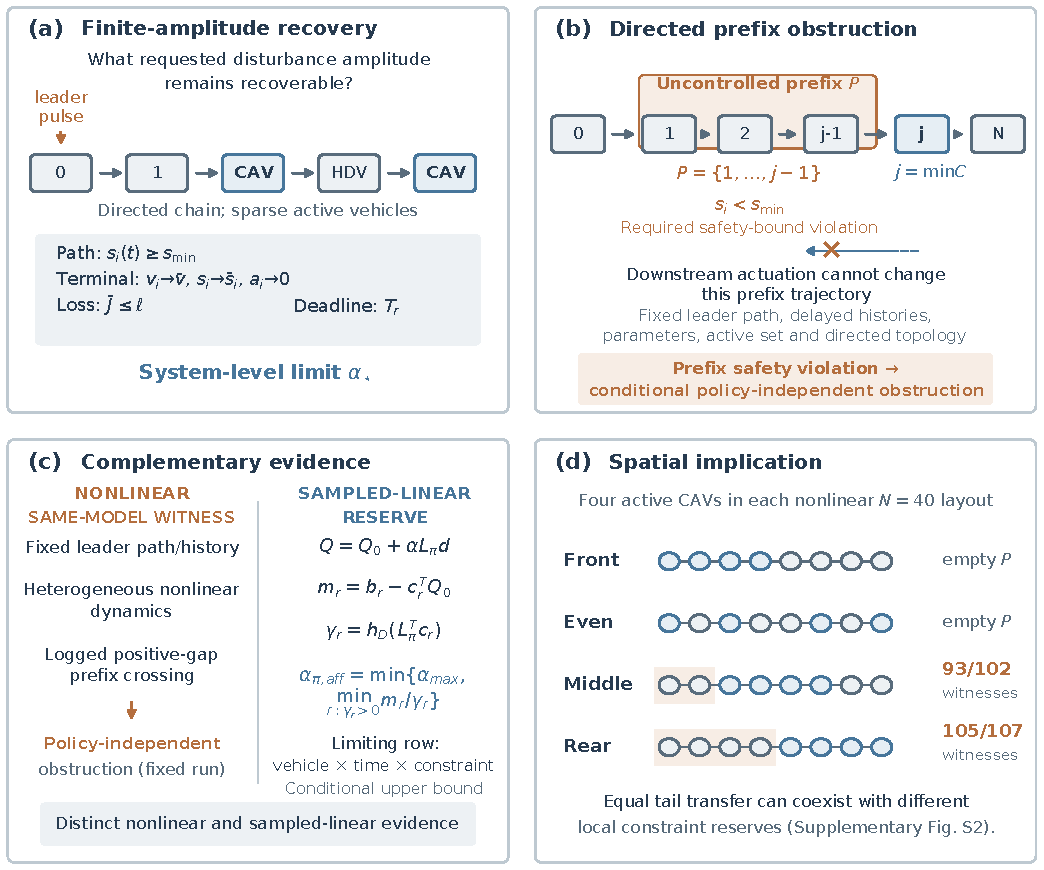
\includegraphics[width=.99\linewidth]{fig1_framework.pdf}
\caption{\textbf{Finite-amplitude recovery and directional obstruction.} (a) Recovery requires path safety, a moving terminal target and bounded distance deficit by a deadline. (b) With fixed leader path, delayed histories, parameters, active set and directed topology, downstream actuation cannot alter a preceding uncontrolled prefix. A crossing below the safety bound obstructs recovery; collision is assessed separately at zero net gap. (c) Nonlinear trajectory witnesses and sampled-linear reserves provide complementary levels of evidence; loss is evaluated separately from the displayed affine-row reserve. (d) Front/even layouts have empty prefixes, whereas middle/rear layouts have nonempty prefixes. The ratios 93/102 and 105/107 are descriptive witness counts among observed failures in the correlated layout grid. Equal scalar tail transfer can coexist with different local sampled-linear reserves (Supplementary Fig.~\ref{SM-fig:tail}).}
\label{fig:framework}
\end{figure}

\subsection*{Collision-aware finite-disturbance recovery}
The primary nonlinear chain contains $N=40$ followers and four active CAVs at indices $\{1,14,27,40\}$. The requested leader pulse has magnitude $\alpha$ in $\mathrm{m\,s^{-2}}$: $-\alpha$ for 1.5 s and $+\alpha$ for 1.5 s, followed by a common return law. Realized acceleration, jerk and speed are constrained. Recovery at 60 s requires all followers to satisfy the specified 4-m minimum net-gap constraint, remain close to the nonzero target speed and gap throughout the final 3 s, and respect a normalized distance-deficit budget of 0.03. Collision is recorded separately at nonpositive net gap.

In the 1,848-run simulation grid, human-only and adaptive-cruise-control traffic had empirical 50\% grid endpoints of $1.0\,\mathrm{m\,s^{-2}}$, and the implemented wave-damping rule reached 1.7. Both endpoint-screened controllers reached the tested $4.5\,\mathrm{m\,s^{-2}}$ ceiling and recovered in 11/12 paired realizations there (Supplementary Table~\ref{SM-tab:nonlinear}). A successful ceiling observation is right-censored: it does not locate the controller's transition.

For illustration, Fig.~\ref{fig:recovery} shows the seed-3 trajectory at requested $\alpha=4.5\,\mathrm{m\,s^{-2}}$. The wave-damping rule first crosses the 4-m safety bound at follower 7 and 17.2 s, then collides at follower 8 and 19.3 s. The speed field ends at collision; both endpoint-screened trajectories recover without collision. Statistical comparisons use the complete simulation grid, and Supplementary Fig.~\ref{SM-fig:constraintuse} shows constraint use in these trajectories.

\begin{figure}[htbp]
\centering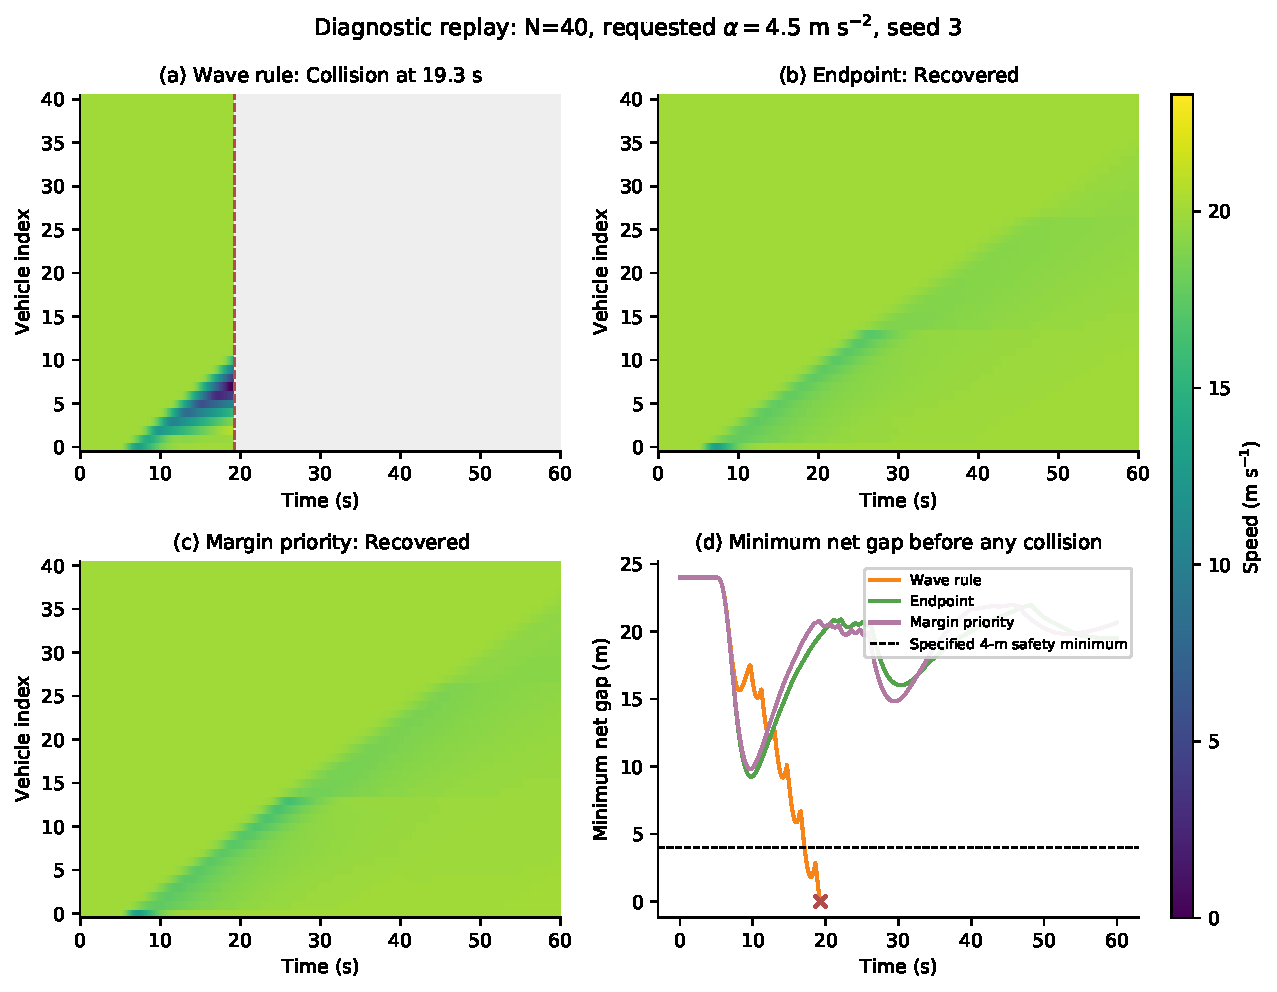
\includegraphics[width=.98\linewidth]{fig1_recovery_collision_aware.pdf}
\caption{\textbf{Representative finite-disturbance trajectories.} (a--c) Speed fields for the wave-damping rule (Wave), endpoint-screened controller (Endpoint) and margin-priority endpoint-screened controller (Margin priority) at $N=40$, requested $\alpha=4.5\,\mathrm{m\,s^{-2}}$ and seed 3. The wave-rule field ends at its first collision (19.3 s). (d) Minimum net gap; the dashed line marks the specified 4-m safety bound. Aggregate outcomes are reported separately.}
\label{fig:recovery}
\end{figure}

\subsection*{A same-model directional obstruction}
Let $\mathcal C$ be the active-CAV index set and $j=\min\mathcal C$. In the predecessor-following chain, the prefix $P=\{1,\ldots,j-1\}$ is independent of policies acting only at $\mathcal C$ when the leader path, delayed histories, parameters and topology are fixed. A required safety violation in $P$ therefore obstructs recovery by controllers behind it (Supplementary Theorem~\ref{SM-thm:prefix}). Supplementary section S7 verifies the corresponding nonlinear trajectory witnesses.

The layout grid fixes $N=40$, four active CAVs, margin-priority endpoint-screened control, IDM followers, an external-leader pulse, 0.7-s human reaction delay, 0.2-s information delay, 0.2-s command delay and 0.35-s actuator time constant; only active positions vary. We classified its declared layout--amplitude--seed cells as A, recovery by this controller; B, its observed failure with a first prefix-safety crossing; C, its observed failure unresolved by the prefix test; or D, not evaluated. These correlated grid-cell counts are descriptive. Among 144 evaluated middle-placement cells, 42 recovered and 102 failed; 93 of the failures have a prefix witness (91.2\%). Rear placement gave 37 recoveries and 107 failures among 144 evaluated cells, with witnesses in 105 failures (98.1\%). Each layout declares 168 cells; middle and rear each lack 24 high-amplitude evaluations. Front placement has 144 recoveries, no observed failure and 24 unevaluated cells; even placement has 167 recoveries and one class-C failure among 168 evaluated cells. Both front and even have an empty prefix, so this particular test supplies no class-B witness for them (Fig.~\ref{fig:obstruction}).

For each class-B cell, the first crossing is a logged positive gap below 4 m at a vehicle in $P$, before any prefix collision. The exact discrete prefix follows the same trajectory under every policy confined to the existing active indices. Class C remains unresolved by this necessary-condition test; D denotes unevaluated cells.

\begin{figure}[htbp]
\centering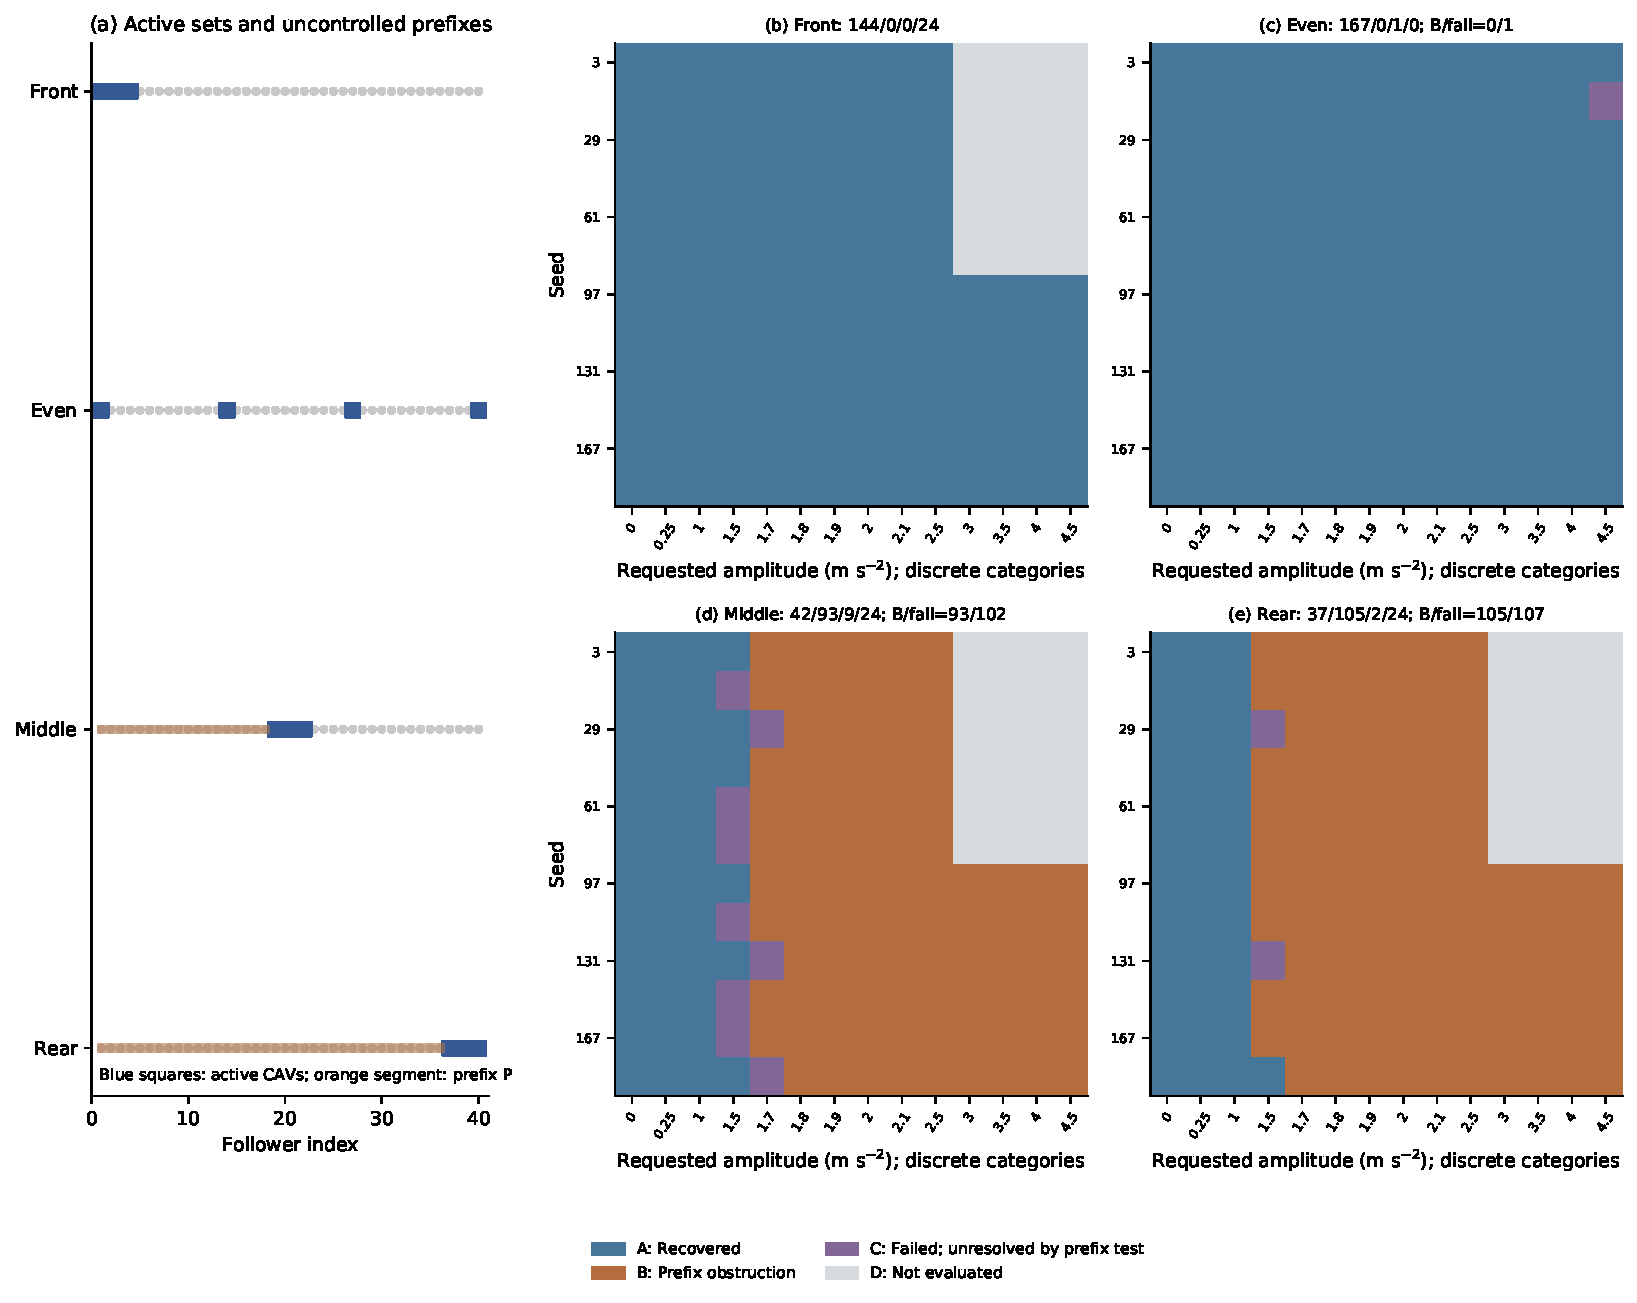
\includegraphics[width=.99\linewidth]{fig2_directional_obstruction.pdf}
\caption{\textbf{Spatial mechanism and nonlinear obstruction classification.} (a) Active indices (blue) and uncontrolled preceding prefixes (orange) for four $N=40$ layouts. (b--e) Seed-by-requested-amplitude outcomes for the margin-priority endpoint-screened controller with IDM followers under the same delays and physical limits. Column spacing is categorical. A denotes recovery, B a prefix-safety witness, C a failed cell unresolved by the prefix test and D an unevaluated cell. Panel titles give A/B/C/D totals and B among observed failures. Exact active indices appear in Supplementary Table~\ref{SM-tab:layouts}.}
\label{fig:obstruction}
\end{figure}

\subsection*{Constraint-resolved sampled-linear limits}
For a fixed sampled-linear model and one implementable affine policy $\pi$, stack all sampled states, commands and terminal quantities in $Q$. Let $W=\alpha Dd$, where $D$ maps dimensionless disturbance coordinates $d\in\mathcal D$ to a unit-amplitude waveform, $\mathcal D$ is compact and contains zero, and $0\le\alpha\le\alpha_{\max}$ is the admitted amplitude range. The nominal response $Q^0$ and unit-amplitude response map $L_\pi$ give
\begin{equation}
Q=Q^0+\alpha L_\pi d,\qquad c_r^\top Q\le b_r .
\label{eq:response}
\end{equation}
Here $c_r$ and $b_r$ are the coefficient and bound of one affine path, command or terminal requirement. For row $r$, define nominal slack $m_r=b_r-c_r^\top Q^0$ and directional support $\gamma_r=h_{\mathcal D}(L_\pi^\top c_r)$, where $h_{\mathcal D}(p)=\sup_{d\in\mathcal D}p^\top d$. If all nominal rows are feasible, the exact affine-row reserve of that fixed policy is
\begin{equation}
\alpha_{\pi,\mathrm{aff}}=\min\left\{\alpha_{\max},\min_{r:\gamma_r>0}\frac{m_r}{\gamma_r}\right\}.
\label{eq:reserve}
\end{equation}
At an equilibrium history with zero nominal speed deficit, let $L_v$ extract follower-speed responses from $L_\pi$, $h$ be the sample interval, $T_r$ the recovery horizon, $N$ the follower count, $\bar v>0$ the target speed and $\ell$ the dimensionless deficit budget. Then the positive-part loss coefficient and full fixed-policy reserve are
\begin{equation}
L_J=\max_{d\in\mathcal D}\frac{h}{N\bar vT_r}\sum_{i,k}[-(L_vd)_{ik}]_+,
\qquad \alpha_\pi=\min\{\alpha_{\pi,\mathrm{aff}},\ell/L_J\},
\label{eq:lossreserve}
\end{equation}
with $[x]_+=\max(x,0)$ and $\ell/L_J=+\infty$ when $L_J=0$. The positive-part loss is evaluated separately for the sampled-linear disturbance family (Supplementary Theorem~\ref{SM-thm:reserve}).

Let $\astar$ denote the supremum of amplitudes for which one causal policy achieves recovery for every admitted parameter and disturbance realization, as defined in Methods. A necessary row in open-loop lifted form is $a_r+p_r^\top U+\alpha d_r^\top d\le b_r$, where $U$ stacks commands and $a_r,p_r,d_r$ are the nominal, control-response and disturbance-response coefficients. If a compact relaxation $\mathcal U_R$ contains the commands of every admissible policy, then
\begin{equation}
\astar\leq \frac{b_r-a_r+h_{\mathcal U_R}(-p_r)}{h_{\mathcal D}(d_r)}
\label{eq:upper}
\end{equation}
whenever the denominator is positive. The numerical example evaluates $p_r=0$; Supplementary Theorem~\ref{SM-thm:upper} covers the general control-response case.

In the 12-follower illustration, the limiting candidate row at 0.2 s common delay is the upper acceleration constraint. Front placement has fixed-policy radius $2.6580\,\mathrm{m\,s^{-2}}$; distributed, middle and rear placements have $2.3772\,\mathrm{m\,s^{-2}}$ and matching prefix bounds. Changing delay alters the limiting vehicle and the front--rear ordering (Fig.~\ref{fig:linear}). Exhaustive evaluation of all 16 disturbance-box vertices agrees with the support calculation (Supplementary Fig.~\ref{SM-fig:vertices}). In this scalar predecessor-following cascade, permuting fixed single-input--single-output (SISO) factors preserves their product and the first-to-last transfer, while local constraint reserves differ (Supplementary Fig.~\ref{SM-fig:tail}).

\begin{figure}[htbp]
\centering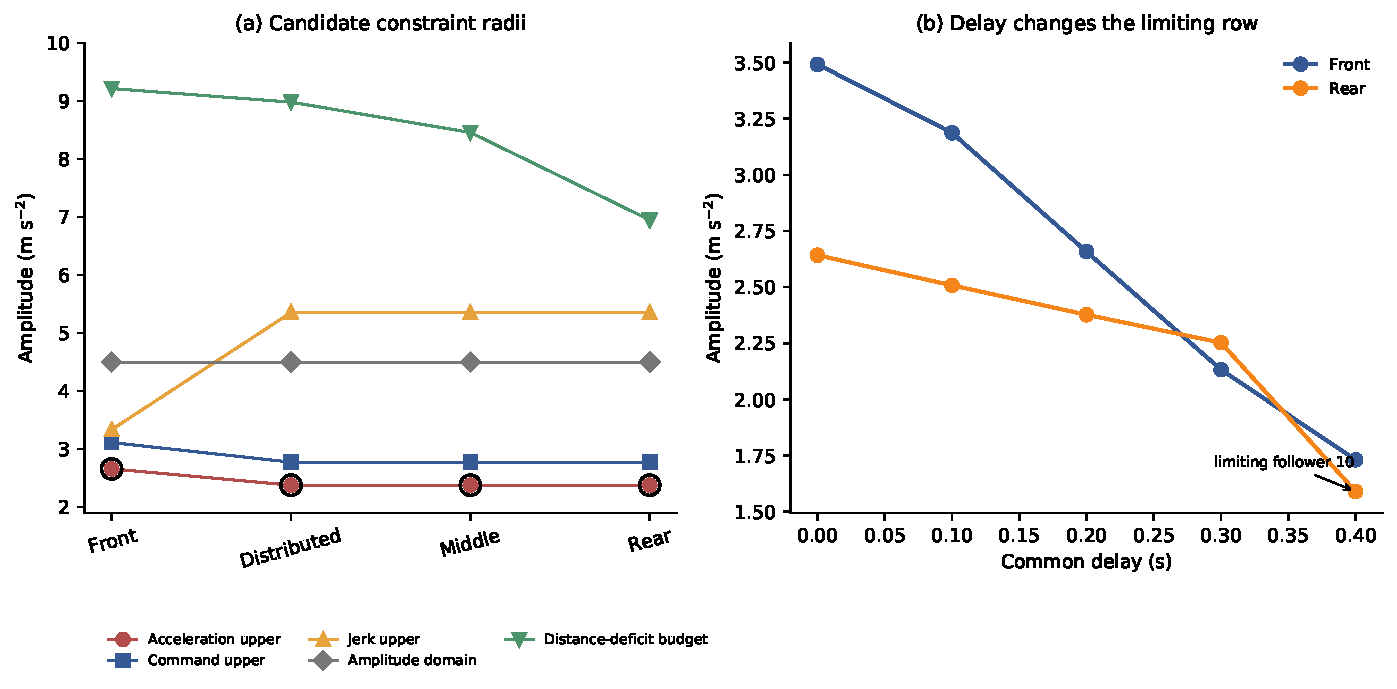
\includegraphics[width=.96\linewidth]{fig3_linear_constraint_rows.pdf}
\caption{\textbf{Constraint-level sampled-linear reserve.} (a) Selected candidate constraint radii at 0.2 s common delay; black rings identify full fixed-policy radii. Values beyond the admitted amplitude domain are analytical continuations. (b) Fixed-policy radii versus common delay for front and rear placements. At 0.4 s the rear limiting row moves to follower 10.}
\label{fig:linear}
\end{figure}

\subsection*{Margin-priority trade-off at the scan ceiling}
The two endpoint-screened controllers use the same candidates, information and physical bounds. Margin priority changes only the secondary selection among commands within 0.01 of the minimum tracking cost. Across 12 paired trajectories at the ceiling, margin priority reduced endpoint gap error in every pair: the median difference was $-1.096$ m, with a seed-bootstrap 95\% interval for the median of $[-1.483,-0.714]$ m. The maximum gap error over the final 3 s also decreased in every pair (median difference $-0.718$ m; interval $[-0.990,-0.436]$ m). Normalized distance deficit increased in every pair (median difference 0.00218; interval [0.00207, 0.00240]) (Fig.~\ref{fig:paired}).

\begin{figure}[htbp]
\centering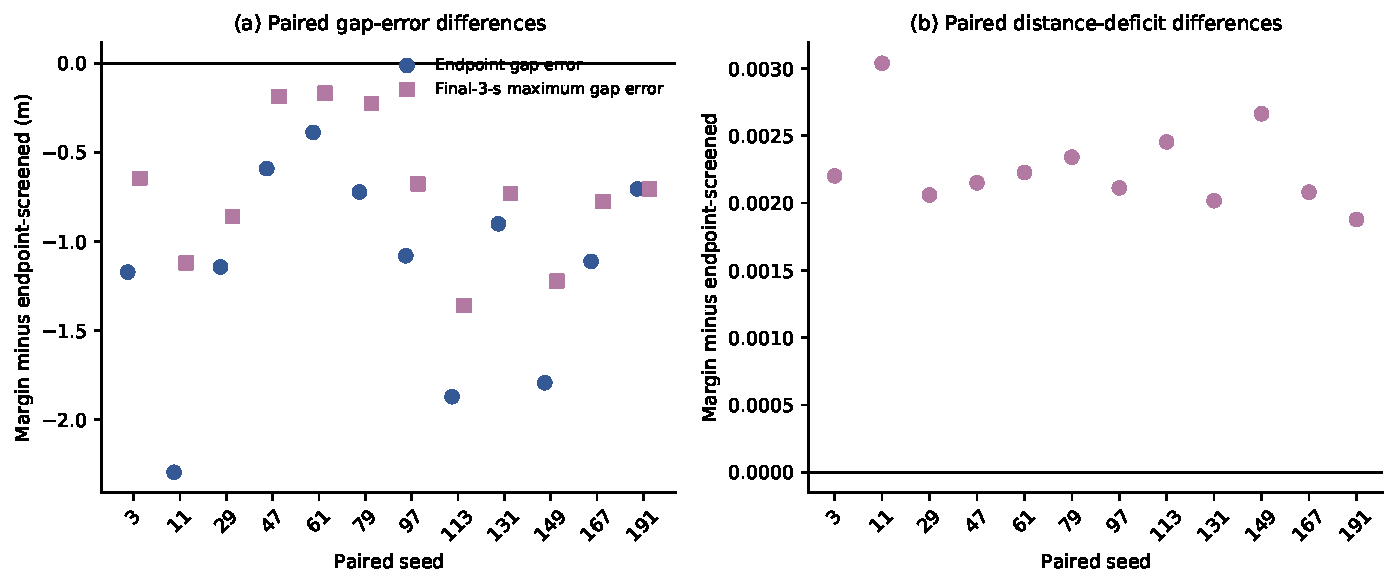
\includegraphics[width=.96\linewidth]{fig4_paired_tradeoff.pdf}
\caption{\textbf{Paired margin-priority trade-off at the scan ceiling.} Differences are margin-priority minus endpoint-screened for the same seed. (a) Endpoint and final-3-s maximum gap-error differences; negative values favor margin priority. (b) Normalized distance-deficit differences; positive values indicate greater loss. All 12 paired differences have the same sign for each outcome.}
\label{fig:paired}
\end{figure}

\subsection*{Cross-model prefix evidence}
A 24-run optimal-velocity/full-velocity-difference (OVM/FVD) extension evaluated middle and rear layouts at requested amplitudes 1.0 and $1.5\,\mathrm{m\,s^{-2}}$ using six paired seeds per condition. Middle placement had three observed failures, all unresolved by the prefix test. Rear placement failed in all 12 runs; three at $1.5\,\mathrm{m\,s^{-2}}$ had a positive-gap prefix crossing below 4 m before any collision (Supplementary Table~\ref{SM-tab:ovm}). The same witness mechanism therefore appears with a second human-driving law, while its occurrence depends on the model and trajectory. These correlated runs probe the mechanism rather than estimate a population frequency.

Source location, finite-horizon disturbance reach and driver-model dependence also affect the interpretation of recovery boundaries (Supplementary Fig.~\ref{SM-fig:scope}).

\FloatBarrier
\section*{Discussion}
The central result separates controller-specific failures from recovery failures imposed by directed topology and path-safety constraints. Ahead of the first active CAV, an uncontrolled prefix follows the same trajectory for every downstream policy under the fixed leader path, histories, parameters and topology. A required safety-bound crossing in that prefix therefore supplies a policy-independent obstruction for the stated run.

Endpoint attenuation cannot resolve this local constraint geometry. In the sampled-linear cascade, permuting fixed scalar follower factors preserves the first-to-last transfer product while changing local vehicle--time--constraint reserves (Supplementary Fig.~\ref{SM-fig:tail}). The nonlinear layout comparison gives the spatial counterpart: with the same vehicle count and controller, placing actuation behind a long uncontrolled prefix exposes upstream safety constraints before downstream inputs can affect them. Sparse placement matters through the position of constrained regions relative to available actuation.

The two evidence layers illuminate this mechanism at different scales. The sampled-linear reserve quantifies limiting vehicle--time--constraint rows and a relaxed upper bound for its stated model and disturbance family. Nonlinear trajectory logs independently establish the observed prefix crossings under the implemented car-following dynamics. Controller comparisons show the practical trade-off between terminal gap error and distance deficit at the tested ceiling.

A low-dimensional directional-feature predictor did not transfer across held configurations (Supplementary Fig.~\ref{SM-fig:predictor}), so structural insight alone does not supply a quantitative boundary model. The present analysis uses synthetic car-following laws, prescribed disturbance families, a fixed single-lane order and a finite horizon. Future work should determine how upstream actuation, communication, lane changes and bidirectional interactions reshape finite-amplitude recovery boundaries.

\section*{Methods}
\subsection*{Recovery problem}
Let $\theta\in\Theta$ denote vehicle parameters, $\PI$ a class of causal policies using only information available at decision time, $\mathcal S$ the path-safe set, $\Erec$ the terminal recovery set and $\bar J$ normalized distance deficit. For nested disturbance sets $\W(\alpha)$ and budget $\ell$, define
\begin{equation}
\astar=\sup\{\alpha:\exists\pi\in\PI\ \forall\theta\in\Theta\ \forall w\in\W(\alpha),\ z(t)\in\mathcal S\ (0\le t\le T_r),\ z(T_r)\in\Erec,\ \bar J\le\ell\}.
\label{eq:systemlimit}
\end{equation}
The policy precedes the uncertain realization in the quantifiers. Here $z$ includes delayed states, $T_r$ is the deadline, and $\Erec$ denotes endpoint tolerances. The nonlinear experiments additionally require these tolerances throughout the final 3 s, a stronger condition. The linear illustration has singleton $\Theta$; nonlinear grid outcomes are controller-specific sampled observations rather than evaluations of Eq.~\eqref{eq:systemlimit} over a continuous uncertainty set.

\subsection*{Nonlinear dynamics and constraints}
Let $s_i$ be follower $i$'s net gap to its predecessor, $v_i$ its speed, and $a_i$ its acceleration. Followers obey $\dot s_i=v_{i-1}-v_i$ and $\dot v_i=a_i$. HDVs use either the intelligent driver model (IDM) \cite{treiber2000congested} or an optimal-velocity/full-velocity-difference (OVM/FVD) law \cite{jiang2001full}, each with 0.7-s reaction delay and independently paired $\pm12\%$ parameter heterogeneity. Parameters are calibrated so that $\bar v=20\,\mathrm{m\,s^{-1}}$ and $\bar s=24$ m are an equilibrium. For CAVs, before clipping,
\begin{equation}
\tau_a\dot a_i=-a_i+u_i(t-\delta_i),
\end{equation}
with $\tau_a=0.35$ s, primary command delay $\delta_i=0.2$ s and separate 0.2-s information delay. Commands are bounded by $[-5,2.5]\,\mathrm{m\,s^{-2}}$, acceleration by $[-4.5,2.0]\,\mathrm{m\,s^{-2}}$, jerk magnitude by $5\,\mathrm{m\,s^{-3}}$, speed by $[0,35]\,\mathrm{m\,s^{-1}}$ and net gap by the specified 4-m safety minimum. Collision is logged at nonpositive net gap.

At each $\Delta t=0.1$-s step, all delayed states are read from a common time-indexed snapshot; follower requests are formed, then saturation, command-delay lookup, actuator lag, jerk and acceleration clipping precede speed, position and gap updates. Newly updated follower states enter only the next step. Speed is projected to its bounds after the acceleration update. A collision flag is recorded at nonpositive net gap; numerical integration then continues for failure accounting, while physical trajectory displays end at collision. Matched controller runs regenerate the same parameter sequence from the same pseudorandom seed.

\subsection*{Nonlinear controllers and endpoint validation}
The adaptive-cruise-control (ACC) command is $k_s(s_i-s_i^{\rm des})+k_v(v_{i-1}-v_i)$ with $s_i^{\rm des}=3\,\mathrm m+(1.05\,\mathrm s)v_i$, $k_s=0.18\,\mathrm{s^{-2}}$ and $k_v=0.75\,\mathrm{s^{-1}}$. The wave-damping baseline adds $(0.35\,\mathrm{s^{-1}})(\bar v-v_i)$ as an implementation-specific speed-restoration term.

Endpoint-screened control enumerates 31 commands $u_j=-5+0.25j$, $j=0,\ldots,30$. At horizon $H=1.2$ s it uses $\rho=1-\exp[-H/\max(\tau_a,\Delta t)]$ and
\begin{equation}
a^+=\operatorname{clip}(a+\rho(u-a),-4.5,2),\quad v^+=v+Ha^+,
\quad s^+=s+H(v_p-v)+\tfrac12H^2(a_p-a^+).
\end{equation}
Here $(s,v,a)$ are the delayed ego net gap, speed and acceleration, $(v_p,a_p)$ those of its predecessor, and $\operatorname{clip}(x,l,u)=\min\{u,\max\{l,x\}\}$. This endpoint-acceleration approximation holds predecessor acceleration constant and does not propagate the queued command delay or jerk sequence. Candidates with $s^+\ge5$ m and $0\le v^+\le35\,\mathrm{m\,s^{-1}}$ form the feasible pool. The 5-m value is a controller screening buffer; the specified safety minimum remains 4 m. If the pool is empty, the implementation reverts to all 31 candidates. The selected command minimizes the dimensionless cost
\begin{equation}
C(u)=\left(\frac{s^+-24\,\mathrm m}{8\,\mathrm m}\right)^2+
\left(\frac{v^+-20\,\mathrm{m\,s^{-1}}}{4\,\mathrm{m\,s^{-1}}}\right)^2+
0.025\left(\frac{u}{1\,\mathrm{m\,s^{-2}}}\right)^2.
\end{equation}
Ascending enumeration breaks exact ties toward the lower command. Here $C_{\min}$ is computed over the feasible pool (or all 31 candidates after the empty-pool fallback). Margin priority uses that same pool and, among candidates with $C\le C_{\min}+0.01$, maximizes the minimum normalized endpoint margin to the specified 4-m gap bound, speed, acceleration and command limits. Thus 5 m controls candidate admission whereas 4 m enters the secondary ranking. Remaining ties use lower cost and then ascending command.

We compared the screening approximation with an exact constant-command first-order-lag endpoint and a discrete held-command counterfactual. The selected command is held for 12 steps after queued commands execute; ego dynamics retain clipping and the predecessor follows its recorded trajectory. Each of 24 paired trajectories contributes 589 eligible time indices and four active vehicles, yielding 56,544 selected-command comparisons. The last 12 indices lack a full 1.2-s horizon; empty-pool counts use the same eligible set. The 95th percentiles of absolute screening-versus-discrete error were 0.0762 $\mathrm{m\,s^{-1}}$ for speed and 0.208 m for gap; the 13,741-decision pulse/command subset reached 2.819 m gap error (Supplementary Fig.~\ref{SM-fig:endpoint}). The counterfactual conditions on the recorded predecessor path.

\subsection*{Disturbance, success and loss}
The requested leader pulse begins at 5 s: $-\alpha$ for 1.5 s, then $+\alpha$ for 1.5 s. Acceleration and jerk constraints shape the realized trajectory, and a gain-$0.8\,\mathrm{s^{-1}}$ return law removes residual leader-speed error. At $\alpha=4.5\,\mathrm{m\,s^{-2}}$ the negative request equals the leader braking bound; the positive request is clipped by the lower positive acceleration limit. Thus $\alpha$ indexes the requested protocol while realized acceleration reflects physical limits.

Recovery requires $s_i\ge4$ m throughout, no collision, and throughout the final 3 s: $|v_i-20|\le1\,\mathrm{m\,s^{-1}}$, $|s_i-24|\le5$ m and $|a_i|\le0.5\,\mathrm{m\,s^{-2}}$. With $[x]_+=\max(x,0)$,
\begin{equation}
\bar J=\frac{1}{N\bar vT_r}\sum_{i=1}^{N}\int_0^{T_r}[\bar v-v_i(t)]_+\,dt\le0.03,
\end{equation}
where $T_r=60$ s and the external leader is excluded. This target-speed distance deficit is evaluated by trapezoidal quadrature on sampled nonlinear speeds; the sampled-linear illustration uses right-endpoint summation. Path safety and recovery are assessed at the reported sample times.

\subsection*{Directional classification and statistical analysis}
For each declared layout-grid cell, category A requires recovery by the evaluated controller. Category B requires failure, nonempty prefix $P$, and a logged first prefix gap below 4 m before any prefix collision; the structural theorem makes this crossing independent of controllers behind the prefix under the stated topology. Category C contains evaluated failures without this prefix witness; they remain unresolved for other admissible controllers. Category D denotes an unevaluated cell. Exact active indices and witness conditions appear in Supplementary Table~\ref{SM-tab:layouts} and section S7; no online reordering is allowed.

The primary grid uses 12 paired seeds. Other placements use 12 seeds through $2.5\,\mathrm{m\,s^{-2}}$ and six at higher amplitudes. Grid endpoints are the largest evaluated amplitude with at least 50\% recovery; ceiling success is reported as censored. Paired contrasts at $\alpha=4.5\,\mathrm{m\,s^{-2}}$ use all 12 paired seeds and 10,000 seed-level bootstrap resamples of the median. Correlated time frames and amplitude cells are not treated as independent samples.

The predictor uses 36 development and 36 configuration-disjoint test records. Its margin feature is the minimum normalized endpoint margin over vehicle, time and constraint at $\alpha=0$; a $0.25\,\mathrm{m\,s^{-2}}$ probe supplies its finite-difference slope. Distance is the absolute index distance from the source to the nearest active CAV. Predictions are clipped to $[0,5]\,\mathrm{m\,s^{-2}}$. Supplementary Fig.~\ref{SM-fig:predictor} reports design rank, conditioning, censoring and configuration-specific errors.

\section*{Data availability}
Numerical source data and simulation outputs supporting this study are available in the public GitHub repository \url{https://github.com/lanston12/directional-recovery-obstructions} and its v1.0.0 release. They include the primary 1,848-run nonlinear study, the separate 24-run OVM/FVD extension, sampled-linear results, representative trajectories, event logs and derived figure-source tables. The repository's source-data inventory maps each display to its numerical sources.

\section*{Code availability}
Custom simulation, verification, analysis and figure-generation code, together with configurations and manuscript sources, is available at \url{https://github.com/lanston12/directional-recovery-obstructions}. The code corresponding to this manuscript is archived in release v1.0.0.

\FloatBarrier
\section*{Supplementary information}
Supplementary Text sections S1--S7; Supplementary Figs.~\ref{SM-fig:vertices}--\ref{SM-fig:scope}; Supplementary Tables~\ref{SM-tab:traceability}--\ref{SM-tab:ovm}.

\bibliographystyle{unsrt}
\begingroup\footnotesize
\bibliography{refs}
\endgroup
\end{document}
